%% LyX 2.3.5-1 created this file.  For more info, see http://www.lyx.org/.
%% Do not edit unless you really know what you are doing.
\documentclass[oneside,UTF8]{ctexbook}
\usepackage[T1]{fontenc}
\setcounter{secnumdepth}{3}
\setcounter{tocdepth}{3}
\usepackage{amsmath}
\usepackage{graphicx}
\usepackage[unicode=true]
 {hyperref}

\makeatletter

%%%%%%%%%%%%%%%%%%%%%%%%%%%%%% LyX specific LaTeX commands.
\newcommand{\noun}[1]{\textsc{#1}}

%%%%%%%%%%%%%%%%%%%%%%%%%%%%%% User specified LaTeX commands.
% 如果没有这一句命令,XeTeX会出错,原因参见
% http://bbs.ctex.org/viewthread.php?tid=60547
% \DeclareRobustCommand\nobreakspace{\leavevmode\nobreak\ }
%%%%%%%%%%%%%%%%%+++++++++++
\usepackage{eso-pic} 
\usepackage{xcolor} % Required for specifying colors by name 
\definecolor{ocre}{RGB}{243,102,25} 
\usepackage{enumerate} 

\usepackage{amsfonts} 
\usepackage{hep} 
\usepackage{bm} 
\usepackage{graphicx,graphics,color} 
\usepackage{simplewick} 
\usepackage{latexsym} 
\usepackage{amssymb} 
\usepackage{makeidx} 
\usepackage{amsmath} 
\usepackage{multirow} 
\usepackage{slashed} 
%%\usepackage[colorlinks,linkcolor=blue]{hyperref} 
%% \usepackage{axodraw2} 
%%++++++++++++++++++++ 
\DeclareMathOperator{\trace}{tr} 
\DeclareMathOperator{\Real}{Re} 
\DeclareMathOperator{\Imag}{Im} 
\newcommand*{\dif}{\mathop{}\!\mathrm{d}}

\makeatother

\usepackage{listings}
\renewcommand{\lstlistingname}{程序列表}

\begin{document}
\title{title}
\author{Thomas Young}

\maketitle
COLLIER is a fortran 单圈-{}-标量和张量的数值积分程序库。 

这些积分出现在微扰的相对论性量子场论中。 

它具有以下features:
\begin{enumerate}
\item 多粒子复杂度 scalar and tensor integrals 
\item ultraviolet divergences 的维数正规化
\item soft infrared divergences 的维数正规化(对于非阿贝尔场,也支持 mass regularization)
\item 对于共线质量奇点的维数正规化或者质量正规化 
\item 对于不稳定粒子,complex 内线质量完全支持(外动量和virtualities认作是实数)
\item 数值危险区域(小 Gram 或者其他运动学行列式),使用专用的展开处理。
\item 所有基本模块都有两种平行的实现方式,可以用作内部交叉检验
\item 缓存系统-{}-用来加速计算 \textbackslash end\{itemize\}
\end{enumerate}
代码提供了量子场论中任意张量和标量积分的数值结果。 
\begin{enumerate}
\item 对于张量积分,不管协变分解中的系数还是张量元本身都将给出。 
\item COLLIER 支持 complex 质量,在计算不稳定粒子时会需要。 
\item 采用维数正规化处理紫外和红外奇点。 
\item 对于 soft 和 共线奇点,有可选用的质量正规化方案。
\end{enumerate}

\chapter{COLLIER doc}

\section{Convention}

一致性地使用 Refs. {[}50, 59{]} 中的约定。约化张量积分的方法在 Refs. {[}43, 50{]} 中有描述,
已经实现4-{}-点函数的结果可以在Ref. {[}59{]}中找到。 标量1-,2-,3-点 函数的结果基于Refs. {[}45,
52{]}

$D$维空间中,单圈$N$点张量积分的一般形式为:
\begin{equation}
T^{N,\mu_{1},\cdots,\mu_{P}}(p_{1},\cdots,p_{N-1},m_{0},\cdots,m_{N-1})=\frac{(2\pi\mu)^{4-D}}{i\pi^{2}}\int\dif^{D}q\frac{q^{\mu_{1}}\cdots q^{\mu_{P}}}{N_{0}N_{1}\cdots N_{N-1}}\label{eq:1}
\end{equation}

其中分母因子 $N_{k}=(q+p_{k})^{2}-m_{k}^{2}+i\epsilon$, $k=0,\cdots,N-1,p_{0}=0$,其中$i\varepsilon$是无穷小的虚部。

对于$P=0$,即分子上是$1$,(\ref{eq:1})定义了$N$-点标量积分$T_{0}^{N}$。 

按照Ref.{[}52{]},我们令$T^{1}=A,T^{2}=B,T^{3}=C,T^{4}=D,T^{5}=E,T^{6}=F,\text{and }T^{7}=G$。

为了能够简洁的写出张量分解。 

我们使用大括号来表示对所有洛伦兹指标进行对称化操作。比如: 

\begin{align}
\{p\cdots p\}_{i_{1}\cdots i_{P}}^{\mu_{1}\cdots\mu_{P}} & =p_{i_{1}}^{\mu_{1}}\cdots p_{i_{P}}^{\mu_{P}}\{gp\}_{i_{1}}^{\mu\nu\rho}=g^{\mu\nu}p_{i_{1}}^{\rho}+g^{\nu\rho}p_{i_{1}}^{\mu}+g^{\mu\rho}p_{i_{1}}^{\nu}\\
{gg}^{\mu\nu\rho\sigma} & =g^{\mu\nu}g^{\rho\sigma}+g^{\mu\sigma}g^{\nu\rho}+g^{\mu\rho}g^{\nu\sigma}
\end{align}

这种分解是可以递归进行的。
\begin{align}
\{p\cdots p\}_{i_{1}\cdots i_{P}}^{\mu_{1}\cdots\mu_{P}} & =p_{i_{1}}^{\mu_{1}}\cdots p_{i_{P}}^{\mu_{P}}\\
\{\underbrace{g\cdots g}p\cdots p\}_{i_{2n+1}\cdots i_{P}}^{\mu_{1}\cdots\mu_{P}} & =\frac{1}{n}\sum\limits _{\substack{k,l=1\\
k<l
}
}^{P}g^{\mu_{k}\mu_{l}}\{\underbrace{g\cdots g}p\cdots p\}_{i_{2n+1}\cdots i_{P}}^{\mu_{1}\cdots\mu_{k-1}\mu_{k+1}\cdots\mu_{l-1}\mu_{l+1}\cdots\mu_{P}}
\end{align}

我们把一般的张量积分约化到洛伦兹协变的结构,as

\begin{align*}
T^{N,\mu1,\cdots,\mu P} & =\sum_{n=0}^{\left[p/2\right]}\sum_{i_{2n+1},\cdots,i_{p}=1}^{N-1}\left\{ \underbrace{g\cdots g}_{n}p\cdots p\right\} _{i_{2n+1}\cdots i_{P}}^{\mu1\cdots\mu P}T_{\underbrace{0\cdots0}_{2n}i_{2n+1\cdots i_{p}}}^{N}\\
 & =\sum_{i_{1},\cdots,i_{p}=1}^{N-1}p_{i_{1}}^{\mu_{1}}\cdots p_{i_{P}}^{\mu_{P}}T_{i_{1}\cdots i_{P}}^{N}+\sum_{i_{3},\cdots,i_{p}=1}^{N-1}\left\{ gp\cdots p\right\} _{i_{3}\cdots i_{P}}^{\mu_{1}\cdots\mu_{P}}T_{00i_{3}\cdots i_{P}}^{N}\\
 & +\sum_{i_{5},\cdots,i_{p}=1}^{N-1}\left\{ ggp\cdots p\right\} _{i_{5}\cdots i_{P}}^{\mu_{1}\cdots\mu_{P}}T_{0000i_{5}\cdots i_{P}}^{N}+\cdots\\
 & +\begin{cases}
\sum_{i_{P}=1}^{N-1}\left\{ g\cdots gp\right\} _{i_{P}}^{\mu_{1}\cdots\mu_{P}}T_{\underbrace{0\cdots0}i_{P}}^{N}, & \text{for }P\text{ odd,}\\
\left\{ g\cdots g\right\} ^{\mu_{1}\cdots\mu_{P}}T_{\underbrace{0\cdots0}_{P}}^{N}, & \text{for }P\text{ even}
\end{cases}
\end{align*}

其中$P/2$是小于等于$P/2$的最大整数。对于洛伦兹协变结构的每一个度规张量,对应的系数携带一个$00$指标,对于每一个动量$p_{i_{r}}$,系数携带一个指标$i_{r}$。通过定义,张量系数$T_{i_{1}\cdots i_{P}}^{N}$对于指标$i_{1},\cdots,i_{P}$
是完全对称的。

UV-{}- or IR-{}-singular 积分利用维数正规化来表示,其中$D=4-2\epsilon$,as, 

\begin{align}
T^{N} & =\tilde{T}_{\mathrm{fin}}^{N}+a^{\mathrm{UV}}(\Delta_{\mathrm{UV}}+\ln\frac{\mu_{\mathrm{UV}}^{2}}{Q^{2}})+a_{2}^{\mathrm{IR}}(\Delta_{\mathrm{IR}}^{(2)}\,\\
 & \,+\Delta_{\mathrm{IR}}^{(1)}\ln\frac{\mu_{\mathrm{IR}}^{2}}{Q^{2}}+\frac{1}{2}\ln^{2}\frac{\mu_{\mathrm{IR}}^{2}}{Q^{2}})+\tilde{a}_{1}^{\mathrm{IR}}(\Delta_{\mathrm{IR}}^{(1)}+\ln\frac{\mu_{\mathrm{IR}}^{2}}{Q^{2}})\\
 & =T_{\mathrm{fin}}^{N}(\mu_{\mathrm{UV}}^{2},\mu_{\mathrm{IR}}^{2})+a^{\mathrm{UV}}\Delta_{\mathrm{UV}}+a_{2}^{\mathrm{IR}}(\Delta_{\mathrm{IR}}^{(2)}+\Delta_{\mathrm{IR}}^{(1)}\ln\mu_{\mathrm{IR}}^{2})+a_{1}^{\mathrm{IR}}\Delta_{\mathrm{IR}}^{(1)}]\label{eq:8}
\end{align}
 其中

\begin{align*}
\Delta_{UV}=\frac{c\left(\epsilon_{UV}\right)}{\epsilon_{UV}}, & \,\, & c\left(\epsilon\right)=\Gamma\left(1+\epsilon\right)\left(4\pi\right)^{\epsilon}\\
\Delta_{IR}^{(2)}=\frac{c\left(\epsilon_{IR}\right)}{\epsilon_{IR}^{2}}, & \,\, & \Delta_{IR}^{(1)}=\frac{c\left(\epsilon_{IR}\right)}{\epsilon_{IR}}
\end{align*}

我们让所有的UV和IR极点清晰的展示出来,包括对应的质量能标$\mu_{UV}$和$\mu_{IR}$。我们进一步提取出因子$c\left(\epsilon\right)=\Gamma\left(1+\epsilon\right)\left(4\pi\right)^{\epsilon}=1+\mathcal{O\left(\epsilon\right)}$,

并把它吸收到$\Delta_{UV}$,$\Delta_{IR}^{(2)},\Delta_{IR}^{(1)}$的定义里。为了避免在(\ref{eq:8})中第一个方程的对数里出现有量纲的量,我们分离出一个辅助的能标$Q$,它隐式地由进入各个圈图的质量和动量决定。

COLLIER的输出对应(\ref{eq:8})的最后一行,包括正比于$a^{UV},a_{2}^{IR},a_{1}^{IR}$的项。参量$\mu_{UV}^{2},\mu_{IR}^{2},\Delta_{UV},\Delta_{IR}^{(2)},\text{and},\Delta_{IR}^{(1)}$可以由用户自由选取,但不会影响UV-和IR-极限下有限的量。

注意我们区分IR和UV起源的奇点,默认$a^{UV},a_{2}^{IR},a_{1}^{IR}$被设置为$0$,输出就是$T_{fin}^{N}\text{\ensuremath{\left(\mu_{UV}^{2},\mu_{IR}^{2}\right)}}$。将$\text{\ensuremath{\Delta\text{'s}}}$设置成不同于$0$的数,可以数值的模拟极点$\epsilon$的影响。

默认IR-和UV-奇点在维数正规化中计算。共线奇点也可以通过质量正规化。为了达到这个目的,相应的质量,下文称为$\overline{m_{i}}$,必须在初始化中被声明为$small$,此外,在后续子程序调用的时候,各质量参数必须和在初始化文件中是精确相同的(但不必要很小)。\emph{小质量}在标量和张量函数中被当作无穷小量对待,其有限值只在质量-奇点的对数项中保留。

阿贝尔类型的软奇点,i.e. 当$a_{2}^{IR}=0$,和共线奇点,通过质量$\overline{m_{i}}$被正规化。当参数$\Delta_{IR}^{(1)}$被设置为$0$之后,参数$\mu_{IR}$可以看作是无穷小的光子或胶子质量。

变动参数$\mu_{UV}^{2},\mu_{IR}^{2},\Delta_{UV},\Delta_{IR}^{(2)},\text{and},\Delta_{IR}^{(1)}$的值可以检查奇点的相消情况。此外,给$\Delta_{UV},\Delta_{IR}^{(2)},\text{and},\Delta_{IR}^{(1)}$选择适合的值,可以允许用户在不同的约定中转换,考虑到提取前置因子$c\left(\epsilon\right)$的不同方式。例如,在\cite{ref61}中,相关的$\epsilon$因子是$\pi^{\epsilon}$,其中$r_{\Gamma}=\Gamma^{2}\left(1-\epsilon\right)\Gamma\left(1+\epsilon\right)/\Gamma\left(1-2\epsilon\right)$,而本文(\ref{eq:1})中的约定为$\left(2\pi\right)^{2\epsilon}$。

因此我们必须如下替换我们的$c\left(\epsilon\right)$:
\[
\frac{c\left(\epsilon\right)}{r_{\Gamma}\left(4\pi\right)^{\epsilon}}=\frac{\Gamma\left(1+\epsilon\right)}{r_{\Gamma}}=\frac{\Gamma\left(1-2\epsilon\right)}{\Gamma^{2}\left(1-\epsilon\right)}=1+\epsilon^{2}\frac{\pi^{2}}{6}+\mathcal{O}\left(\epsilon^{3}\right)
\]
为了得到\cite{ref61}中约定下的奇点积分。这等价于作替换$\Delta_{IR}^{\left(2\right)}\rightarrow\Delta_{IR}^{\left(2\right)}+\pi^{2}/6$,同时保持我们计算中的$\Delta_{UV}\text{and}\Delta_{IR}^{\left(1\right)}$不变。在此变换之后,我们的参数$\Delta_{UV},\Delta_{IR}^{(2)},\text{and},\Delta_{IR}^{(1)}$就分别对应于文献\cite{ref61}中的极点$1/\epsilon,1/\epsilon^{2},\text{and}1/\epsilon$。

\subsection{总结}

对于单圈$N$点张量积分:
\[
T^{N,\mu_{1},\cdots,\mu_{P}}(p_{1},\cdots,p_{N-1},m_{0},\cdots,m_{N-1})=\frac{(2\pi\mu)^{4-D}}{i\pi^{2}}\int\dif^{D}q\frac{q^{\mu_{1}}\cdots q^{\mu_{P}}}{N_{0}N_{1}\cdots N_{N-1}}
\]

点的数目是$N$,那么引入的外动量数目是$N-1$,最后张量指标的数目也是$N-1$。依照惯例,把分子上不含积分动量的积分称为标量积分$A,B,C\cdots,G$,

一个张量积分可以约化成 coefficients and 张量结构的形式。coefficients就是一些含有不同外动量参数的标量积分$A,B,C\cdots,G$,张量结构由外动量的对称化和度规张量组成。张量结构中外动量的对称性,可以从积分表达式中看出来。

\section{introduction}

multi-leg one-loop amplitudes 振幅求值的巨大进步,来自于两方面:
\begin{enumerate}
\item 传统费曼图方法的系统改进 
\item 基于推广的幺正性关系的新理论技术
\end{enumerate}
在第二种方法中,单圈振幅被直接表示成标量积分的组合。 这种向固定标量积分基的直接约化,会引发相空间特定区域的数值问题。 一般可以通过采用四次精度的数值计算克服。

相反,费曼图方法,包括最近的递归方法依赖于张量积分。 此方法允许分解方法自适应于相空间的不同区域,在相当大的程度上, 通过最优选择避免数值不稳定性。
COLLIER 库提供了计算标量和张量积分的全面工具。 在两种互补的方法中都能应用。

将张量积分约化到一小族基本积分的方法,可以追溯到 Brown and Feynman, Melrose, and Passarino
and Veltman。 又经过了数十年的发展,文献{[}43, 50{]} 展示的完整方法,是COLLIER代码的基础。 作为张量分解基础的标量积分首次由t'
Hooft and Veltman 进行了系统研究。 已经存在数个计算单圈标量和张量积分的库,比如:
\begin{itemize}
\item FF,LoopTools, 
\item QCDLoop,OneLoop, 
\item GoLem95C,PJFRY,Package-X
\end{itemize}
这里介绍的COLLIER库,提供完全的张量积分集合,处理带有复数质量的过程, 并且没有先验的粒子数限制。

COLLIER 已在用于多个前沿课题的计算。

文章结构:
\begin{itemize}
\item Section 2: COLLIER相关约定 
\item Section 3:计算张量积分的方法轮廓 
\item Section 4:COLLIER 库的内部结构
\item Section 5: 用法
\item Section 6:总结 
\item Appendix A:定义 单圈积分的 运动学输入细节
\end{itemize}

\section{实现方法}

\subsection{张量系数的计算}

计算张量积分的方法依赖于它的传播子数目$N$。对于$N=1,2$,我们使用显式的数值稳定表达式\cite{ref37,ref50}。

对于$N=3,4$,所有张量积分被数值约化到基本的标量积分,通过使用文献\cite{ref45,ref52,ref59}给出的解析表达式。默认情况下,约化使用的是标准的
\noun{Paassarino-Veltman} \cite{ref37}约化。在相空间不稳定殿,其 \noun{Gram} 行列式变得很小,\noun{Paassarino-Veltman}
约化变得不稳定。这在些点上,我们使用专用的递归展开方法\cite{ref50}。所有这些方法都在COLLIER中得到实现,并且对于展开参数可以到任意阶。为了决定一个特定相空间点的约化方法,以下步骤被采用:
\begin{enumerate}
\item 默认是 \noun{Passarino-Veltman} ,它的可靠性通过一个给标量积分预先分配的精度来估计,然后估计约化时的误差传递。如果积分最高rank$\hat{P}$的最终的误差结果$\Delta T^{N}\left(\hat{P}\right)$,小于一个预定义的精度标签$\eta_{\text{req}}$(required
precision),结果被保留并传递给用户。
\item 若步骤1没有提供足够的精度,一般意味着张量积分包括外动量的小 \noun{Gram} 行列式。COLLIER 切换到专用展开。为决定到哪一阶是足够的,一个先验的误差估计式$\Delta T_{\text{prelim}}^{N}\left(P\right)$,对于系数$T_{i1,\cdots iP}^{N}$被构建,对于不同方法的最高rank$\hat{P}$。误差估计基于展开的期望精度评定,和所需标量积分的简化的误差传递。$\Delta T_{\text{prelim}}^{N}\left(P\right)$最小的展开方法被采用。在展开式的实际计算中,评估的是更加现实的精度$\Delta T^{N}\left(P\right)$,通过分析最后一次迭代的修正。如果预定义的精度标签$\eta_{\text{req}}$达到,结果被保存并返回给用户。否则在达到一个预定义的展开深度时,展开停止,或者从一次迭代到下一次,精度没有增加。
\item 如果步骤2没有提供所需精度。将对其他方法进行重复,这些方法对于足够小的$\Delta T_{\text{prelim}}^{N}\left(P\right)$,将能够保证收敛。如果经过这些重复任一个,达到预定义精度,结果被保留并返回给用户。
\item 如果\noun{ Paassarino-Veltman }和其他展开方法都不能达到目标精度,具有最小误差估计的$\Delta T^{N}\left(P\right)$的方法,其结果将被返回给用户。
\end{enumerate}
通过这种方法,对于几乎所有相空间的点,都能得到稳定的结果。保证了可靠的 \noun{Monte Carlo 积分。}

对于$N=5,6$,张量积分被约化到具有更低rank和$N$的积分,遵循\cite{ref50,ref43},i.e. 不涉及到
\noun{Gram 行列式的逆。对于$N\geq7$,}文献\cite{ref50}Section 7中$6$–点张量积分约化的修改版被应用(见$\left(7.10\right)$之后的文字)。

\subsection{全张量的计算}

目前为止,文中描述的方法是用洛伦兹不变的项进行约化,得到的系数为$T_{i1,\cdots,iP}^{N}$。新一代的NLO生成器比如
\noun{OPENLOOPS}, \noun{RECOLA,}需要全张量$T^{N,\mu1,\cdots,\mu P}$的分量。为了达到这个目的,COLLIER
中实现了一套高效的算法,来从$T_{i1,\cdots,iP}^{N}$构建$T^{N,\mu1,\cdots,\mu P}$。它递归地计算4中那些单举动量构造的张量结构。张量结构的非零分量包括度规矩阵递归地得到,通过添加成对相等的洛伦兹指标,到带有更少度规的张量上,考虑到指标组合因子和度规张量引起的符号。相关的组合系数在COLLIER
初始化的时候计算并列表。

洛伦兹不变的系数$T_{i1,\cdots,iP}^{N}$和$T^{N,\mu1,\cdots,\mu P}$被列在fig.\ref{fig:1}中.

\begin{figure}
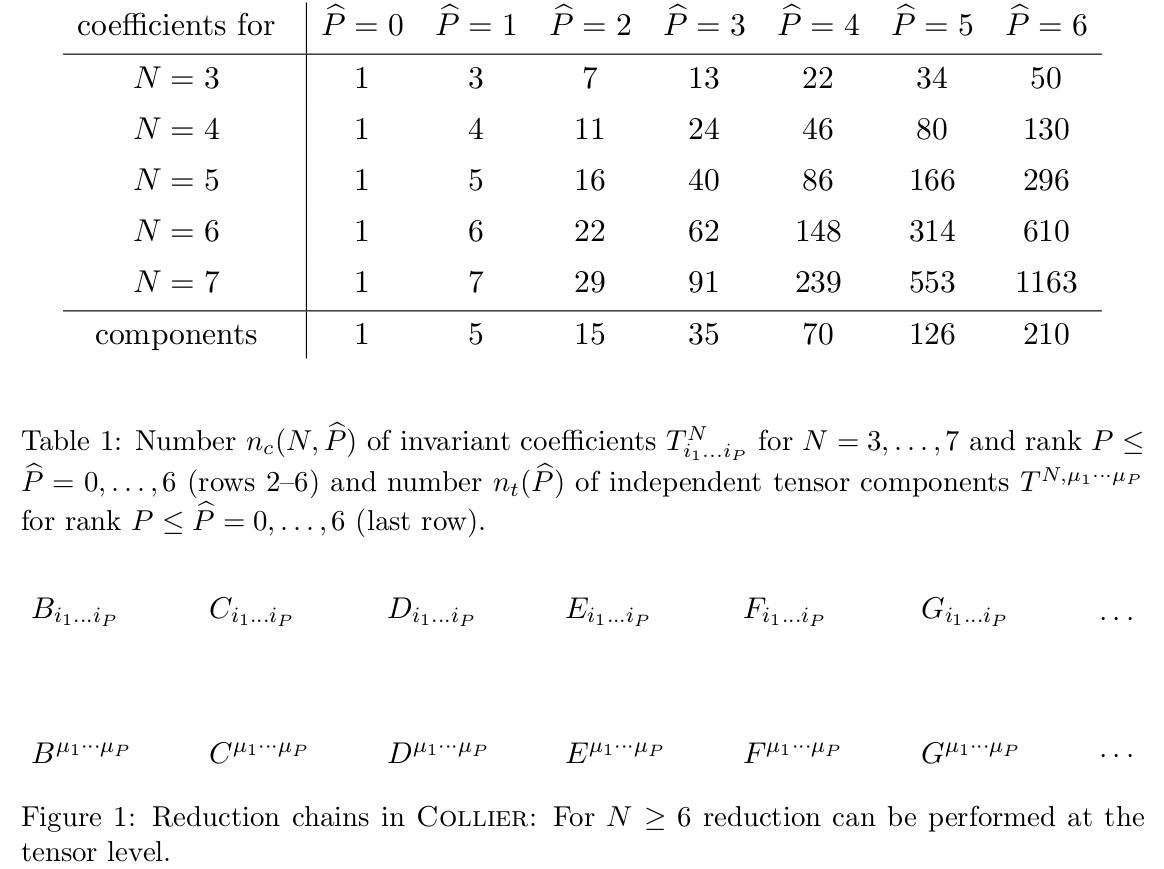
\includegraphics[scale=0.48]{pasted10}

\caption{COLLIER 约化链:对于$N\protect\geq6$,约化可以在张量层次进行\label{fig:1}}
\end{figure}

\noun{对于$N\leq4$,}不变系数的数目小于张量分量的数目\noun{,}这也是 Passarino-Veltman 约化方法的前提。另一方面,对于$N\geq5$,情况发生反转。实际上,\cite{ref50}中$(7.7)$中对于$N\geq6$所展现的方法,约化是用全张量的项推导的。若要得到张量系数,需要进行对陈化操作,得到的系数也不是唯一的,由于张量结构具有的冗余性。所以,对于$N\text{\ensuremath{\geq}6}$的张量$T^{N,\mu1,\cdots,\mu P}$的约化,COLLIER
直接在张量层次实现,而不用依赖于协变分解。

而当$N\leq5$,迭代在coefficient 的层次 exclusively 进行,$T^{N,\mu1,\cdots,\mu P}$随后才构建,由各自的
coefficients $T_{i1,\cdots,iP}^{N}$ ,对于$N\text{\ensuremath{\geq}6}$,约化也可以在tensors层次完成。意思是,若要计算一个$N\text{\ensuremath{\geq}6}$的张量积分,可以选取一个$5<N_{\text{tenred}}\leq N$的$N_{\text{tenred}}$,对于$N<N_{tenred}$,进行coefficients
层次的递归运算,对于$N\text{\ensuremath{\geq}}N_{tenred}$,在tensor 水平进行计算。从
coefficients 到 tensor 的转变可以发生在$N_{\text{tenred }}-1$。可能的约化链示于图\ref{fig:1}。

\section{库的结构}

COLLIER 的结构在图2中图形化的展示出来。库的核心由模块 COLI 和 DD 组成。它们是标量积分$T_{0}^{N}$和洛伦兹不变系数$T_{i_{1}\cdots i_{P}}^{N}$的两种独立的实现,利用前文描述的方案。模块
\emph{tensors} 提供了从$T_{i_{1}\cdots i_{P}}^{N}$构建$T^{N,\mu_{1}\cdots\mu_{P}}$的路径,同时也包括$N\geq6$的时候$N$点积分,张量层次的直接约化。用户通过COLLIER的全局界面和COLI,DD,and
tensors 的常规流程交互。它提供了路径,去设置或提取 COLI 和 DD 的参数,还有计算张量系数$T_{i_{1}\cdots i_{P}}^{N}$和张量元$T^{N,\mu_{1}\cdots\mu_{P}}$的路径。用户可以选择使用那个分支–COLI或DD。也可以用两个分支计算每个积分,来做结果的交叉检验。

在计算一个典型的单圈矩阵元时,一个张量积分会被调用好几次,并输入相同的运动学参数:另一方面,在计算$P\geq2$的$N$点积分时,会引起对更低阶$N\prime$积分的递归调用。在约化树中,对于$N\prime\leq N-2$阶的积分,有不同的抵达路径。为了避免对同一个积分进行重复运算,COLLIER
的子库连接到了一个Global的cache系统,其工作原理如下:

参数$N_{\text{ext}}$计数外部程序的积分调用次数,在约化过程中,内部调用被一个二进制标识符$id$记录。对于每一个索引对$\left(N_{\text{ext,}}id\right)$分配一个指针。对于第一个相空间点的计算,相应函数的参数被比较,具有相同参数的索引对$\left(N_{\text{ext,}}id\right)$被指向cache中的相同地址。第一次计算的结果被写入cache,后续相空间点的计算可以读取这些结果,如果指向相同的地址。使用external
cache 系统是可选择的,在一个 Monte Carlo 积分中,对张量积分的调用,需要相空间所有点的次序是exactly相同的,在初始化之后(初始化标志着矩阵元计算的开始,对于各个相空间点)。此外,对于每个事件,第一次和最后一次调用积分的内部参数必须保持不变。

\section{库的使用}

\subsection{安装}

下载包 COLLIER-$v$.tar.gz \href{http://collier.hepforge.org}{collier homepage}。其中$v$是库的版本。还应该安装CMAKE创建系统。由于COLLIER是一个单机的
Fortran95 代码,无需额外的库。

gunzip and untar COLLIER-v.tar.gz 将会解压到 ./COLLIER-$v$ 文件夹,包含以下文件和文件夹
\begin{enumerate}
\item Cmakelists.txt :cmake makefile 用来产生COLLIER 库。
\item src:COLLIER 源代码库,包含COLLIER的主要代码和子库的主要代码。
\begin{itemize}
\item COLI:包含COLI分支的文件
\item DDlib:包含DD分支的文件
\item tensors:包含构建张量和直接张量约化的文件
\item Aux:包含辅助文件。
\end{itemize}
\item build:build 文件夹,CMAKE 存放所有创建用必须文件的地方,比如对象文件。
\item modules:空文件夹,for fortran 模块文件。
\item demos:展示COLLIER 用法的示例文件夹。
\item COPYING:版权信息文件。
\end{enumerate}
使用以下命令创建COLLIER库:

\begin{lstlisting}
cd build
cmake 
make
\end{lstlisting}

默认cmake会建立一个动态库。如果需要静态库,在 COLLIER-v 文件夹中,使用以下选项

\begin{lstlisting}
cmake -Dstatic=ON ..
\end{lstlisting}

如果不指定编译器,cmake会自动寻找安装的fortran编译器,选择合适的。使用特定的编译器比如 ifort,可以用以下选项

\begin{lstlisting}
cmake -DCMAKE_Fortran_COMPILER=ifort ..
\end{lstlisting}

可以给出编译器的全路径。

makefile创建以后,make命令就会产生动态库 libCOLLIER.so 或者静态库 libCOLLIER.a 在COLLIER-v
文件夹中,可以用来链接到用户程序。

若要创建demos 文件夹内示例程序的可执行文件,在文件夹COLLIER-v/build 内使用

\begin{lstlisting}
make demo
make democache
\end{lstlisting}

所有使用make 命令创建的文件可以用 ``make clean''来丢弃,在 COLLIER-v/build 中来运行。

也可以删除 COLLIER-v/build 中的所有文件。

\rule[0.5ex]{1\columnwidth}{1pt}

Sample programs

在COLLIER-v/build 文件夹中使用以下命令创建两个示例程序
\begin{lstlisting}
make demo
make democache
\end{lstlisting}
可以在COLLIER-v/demo 文件夹使用以下命令运行
\begin{lstlisting}
./demo
./democache
\end{lstlisting}

程序 demo 专门用来计算single张量积分。

在运行过程中,会询问用户在$N$点-积分中选择一个例子来计算。计算结果被写入 demo\_Npoint\_exampleX.dat
中,它指向 demo.f90 中的段落,其中给出了计算各个积分的源代码,接着一小段程序,用来给COLLIER输出化,对于所有示例程序都差不多。其中包含了很多被注释的行,去掉感叹号就会起作用,其中展示了很多COLLIER的global参数,可以修改使用。

程序decmocache 展示了cache 的用法。对于1000个相空间点,8个张量积分被计算了数次。这个玩具 monte carlo
在四种子集中相继执行: 先用 COLI,用或不用缓存,再用DD,用或不用缓存。源代码存储在文件 democache.f90 中。

\subsection{概括使用说明\label{subsec:=006982=0062EC=004F7F=007528=008BF4=00660E}}

为了在FORTRAN程序中使用 COLLIER, COLLIER-$\nu$/modules 中的对应模块 必须被载入:

\begin{lstlisting}
use COLLIER
\end{lstlisting}

COLLIER-$\nu$中的\emph{library libCOLLIER.so} or \emph{libCOLLIER.a}
必须提供给\noun{linker}。这样程序才有权访问COLLIER的公共函数和子程序。所有的子程序都带有后缀''\_cll''。为了避免冲突,也为了增加可读性。

在使用COLLIER之前,必须进行初始化,Calling

\begin{lstlisting}
subroutine Init_cll(Nmax,rin,folder_name,noreset)
integer Nmax :maximal # of loop propagators
integer, optional rin :maximal rank of loop integrals
character, optional folder_name : name of folder for output
logical, optional noreset : no new output folder and files
\end{lstlisting}

\texttt{Nmax} 是强制性的,另外两个参数 \texttt{rin},\texttt{folder\_name}, and
\texttt{noreset} 是可选的。利用Nmax指定所需计算张量圈积分$T^{N,P}$的最大传播子数目。($N<N_{max}$),可选参数
rin 制定了 最高阶 $P_{max}(p\le P_{max})$。如果参数 rin 被忽略,那么默认将rin设置为 Nmax,对于可重整化理论足够。Nmax
and rin 决定了COLLIER 内部产生的表格的大小。

folder\_name 参数指定特定名称的输出文件夹。缺省值是 'output\_cll'。也可以传递给 init\_cll 一个空字符串foldername='',这样会阻止创建输出文件夹,除了初始化信息和重要错误会被写入到标准输出通道
stdout\_cll=6.

在后续的调用和计算中,如果 noreset 被设置为 .true., 那么输出文件夹不会被重新创建,但是文件会被覆盖。在第一次call
init\_cll 的时候,flag noreset 会被忽略。

call init\_cll 会将所有内部参数设置为 Table.\ref{fig:Table-2:-lists} 中的值。在后续的调用中,如果
noreset设置为.true.,那么自行设定的参数值不会被重置为这里的初始化值。

\begin{figure}
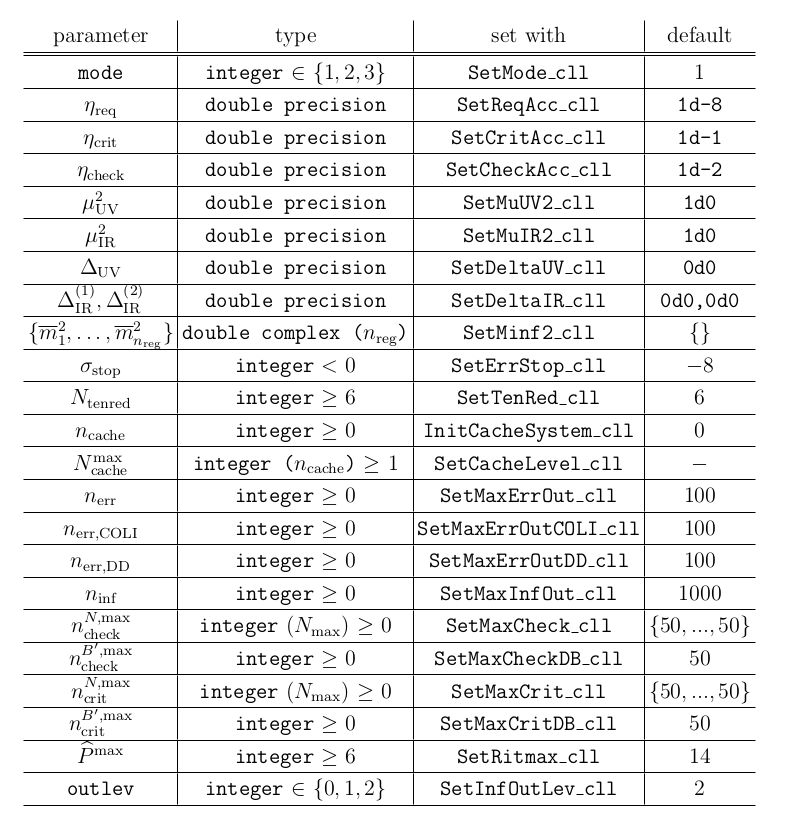
\includegraphics[scale=0.8]{pasted2}

\caption{Table 2: lists of COLLIER parameters\label{fig:Table-2:-lists}}
\end{figure}

在初始化之后,很多参数可以被设置得不同,满足用户需要。为实现这个功能,COLLIER 提供了subroutine SetX\_cll
对每个参数 X,subroutines SwitchOnY\_cll, SwithchY\_cll,对于每个 flag Y。To read
out the current value of parameter X, a subroutine getX\_cll is available.
这些参数可以被用户修改,subroutine 在 section5.4 进了详细描述。

在初始化之后和可能潜在的重新定义之后,COLLIER 就可以计算张量积分了。

通用subroutine TN\_cll 计算洛伦兹协变分解中的张量系数 $T_{i1,\cdots,iP}^{N}$

TNten\_cll 返回张量元 $T^{N,\mu1\cdots\mu p}$。

此外也提供可选的特定 subroutine A\_cll, B\_cll,...,\textbackslash G\_cll, and
Aten\_cll, Bten\_cll,..., Gten\_cll for the 1-,2-,...,7-point 积分,同样也有
A0\_cll, B0\_cll, ..., D0\_cll 对于标量积分。

两点函数的动量导数,通常需要用来计算重整化常数,可以使用通用subroutine DB\_cll 计算到任意阶。对于最低阶,可以使用特定
subroutine, DB0\_cll, DB1\_cll, DB00\_cll, and DB11\_cll。更多介绍张量积分计算
subroutine 的信息在 section5.3 中给出。

COLLIER 的一个典型应用是在一个 NLO Monte Carlo 生成器中,提供单圈张量积分。在这种情况下,主程序对 MC 事件进行一个循环,对于每个事件,主程序调用COLLIER计算一组张量积分来得出矩阵元。在这种情形下中,the
subroutine

\begin{lstlisting}
subroutine InitEvent_cll(cacheNr)
integer, optional cacheNr: number of cacher
\end{lstlisting}
应该在每次计算张量积分之前被调用。这个调用将初始化error flag and accuracy flag of COLLIER,这些flag可以在积分计算完成后,读取用来得到计算status
的 整体信息。如果使用了 cache system,call of InitEvent\_cll 将是必须的,以用来初始化每次 MC
事件的 cache。如果使用了 multiple caches,那么各自的 cache number \texttt{cacheNr
}需要传递给 \texttt{InitEvent\_cll}, 作为一个可选参数。更多关于使用缓存的信息,可以在 section5.5
中找到。

为了帮助用户熟悉COLLIER的使用,两个示例程序demo和democache一并包含在发行版中。在 section 5.7 中可以找到描述。

\subsection{张量积分的计算}

对于张量积分,COLLIER提供了subroutine,传递洛伦兹协变分解系数$T_{i1,\cdots,ip}^{N}$,和张量元$T^{N,\mu_{1},\cdots,\mu_{P}}$。

\begin{equation}
T^{N,\mu_{1},\cdots,\mu_{P}}(p_{1},\cdots,p_{N-1},m_{0},\cdots,m_{N-1})=\frac{(2\pi\mu)^{4-D}}{i\pi^{2}}\int\dif^{D}q\frac{q^{\mu_{1}}\cdots q^{\mu_{P}}}{N_{0}N_{1}\cdots N_{N-1}}\label{eq:1-1}
\end{equation}

积分中的外部变量共$N-1$个,分子上的带指标被积动量共有$p$个。所以出来的洛伦兹结构中,也是有$p$个指标,

构成这$p$个指标的材料为,度规张量和$N-1$个外动量,从中挑选出$p$个,所以外动量的循环指标是$1\sim N-1$.

其中分母因子 $N_{k}=(q+p_{k})^{2}-m_{k}^{2}+i\epsilon$, $k=0,\cdots,N-1,p_{0}=0$,其中$i\varepsilon$是无穷小的虚部。

\begin{align*}
T^{N,\mu1,\cdots,\mu P} & =\sum_{i_{1},\cdots,i_{p}=1}^{N-1}p_{i_{1}}^{\mu_{1}}\cdots p_{i_{P}}^{\mu_{P}}T_{i_{1}\cdots i_{P}}^{N}+\sum_{i_{3},\cdots,i_{p}=1}^{N-1}\left\{ gp\cdots p\right\} _{i_{3}\cdots i_{P}}^{\mu_{1}\cdots\mu_{P}}T_{00i_{3}\cdots i_{P}}^{N}\\
 & +\sum_{i_{5},\cdots,i_{p}=1}^{N-1}\left\{ ggp\cdots p\right\} _{i_{5}\cdots i_{P}}^{\mu_{1}\cdots\mu_{P}}T_{0000i_{5}\cdots i_{P}}^{N}+\cdots
\end{align*}

张量系数$T_{i1,\cdots,ip}^{N}$表示成一个N–维数组,type double complex, 并按照如下的约定:

\[
TN\left(n_{0},n_{1},\cdots,n_{N-1}\right)=T_{\underbrace{0\cdots0}_{2n0}\underbrace{1\cdots1}_{n1}\underbrace{2\cdots2}_{n2}\underbrace{N-1\cdots N-1}_{nN-1}}^{N}
\]

利用这种方法,所有张量系数,$T_{i1\cdots iP}^{N}$,其中$P=0,\cdots\hat{P}$, up to
a given rank $\hat{P}$, 可以储存进同一个数组中

$\text{\text{double complex }TN}(0:[\hat{P}/2],\underbrace{0:\hat{P},\cdots,0:\hat{P}}_{N-1})$

注意到相同的系数$T_{i1\cdots ip}^{N}$,通过一个指标的置换$\left\{ i1,\cdots,iP\right\} $相互关联,在
\texttt{TN }中也被表示成同一个 entry。作为例子,张量系数$D_{i1..iP}$和数组 \texttt{D }的对应关系,展现在
Table.\ref{fig:table-3} 中。这是$4$点函数到阶数$4$的情形。

圈积分$D$有$4$个传播子,$3$个外动量,所以允许的最高阶指标数目为$4$,

左边一列的下标中的数字,指的是传播子中外动量的序号,在结果中出现。重复的表示重复出现。

右边一列的四个位置,相当于四个传播子,其中的数字,是每个外动量,在最终结果中出现的次数。

它们是一一对应的。

\begin{figure}
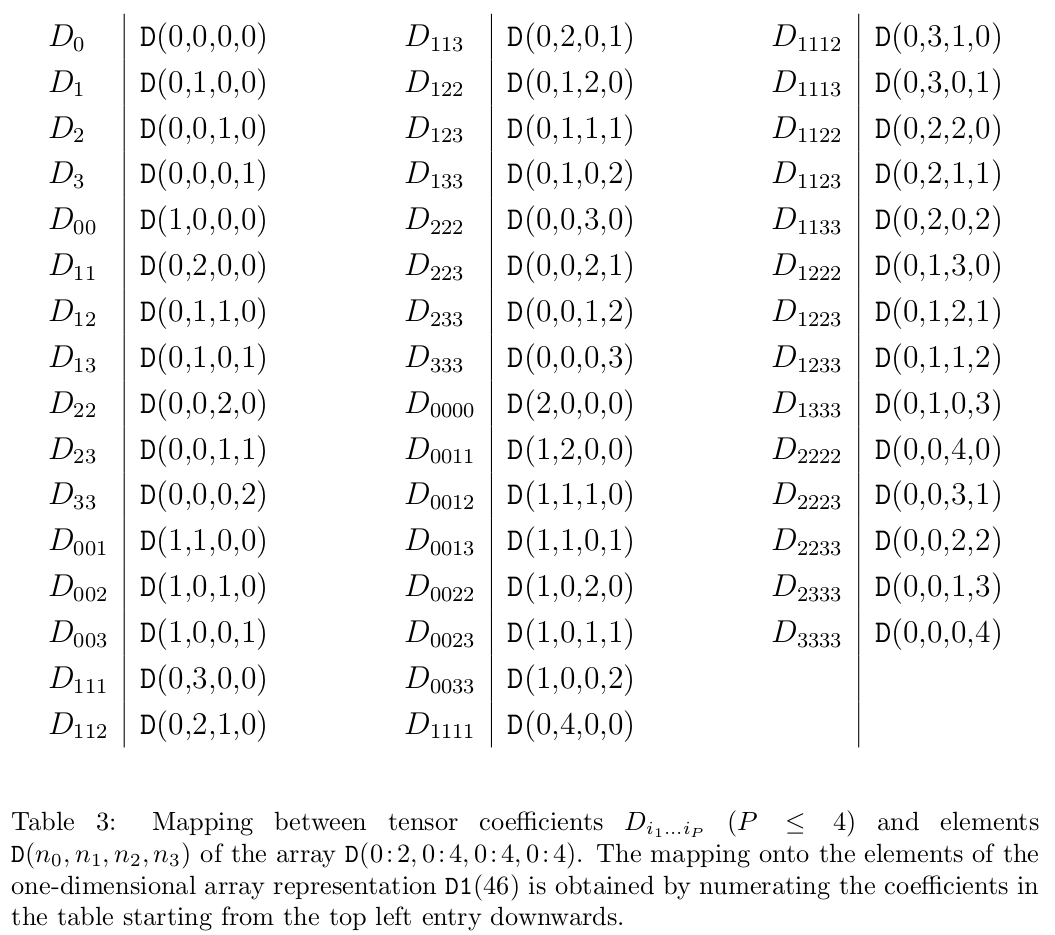
\includegraphics[scale=0.52]{pasted3}

\caption{table 3 \label{fig:table-3}}
\end{figure}

可选的,N-点积分的张量系数up to rank $\hat{P}$,可以通过一维数组得到

\[
\text{double complex TN1}\left(\eta_{c}\left(N,\hat{P}\right)\right)
\]

其中$\eta_{c}\left(N,\hat{P}\right)$是张量系数$T_{i1\cdots iP}^{N}$的总数目,其中$i1\leq i2\leq\cdots\leq iP\text{ and }P\leq\hat{P}$。对于$N=1,\cdots,7$
and $\hat{P}=0,\cdots6$,$\eta_{c}\left(N,\hat{P}\right)$的具体数值在 table.\ref{fig:table-1}
中给出。张量系数在数组 \texttt{TN1 }中按照 升序排列,从$P=0$到$P=\hat{P}$。相同rank的系数$T_{i1\cdot iP}^{N}$和$T_{j1\cdots jP}^{N}$按照他们的第一个相异的指标$i_{k},j_{k}$进行排列。对于$4$点函数至rank$4$,排序表见于\ref{fig:table-3}。由于
FORTRAN 数组只支持到$7$维,所以,对于$N\ge8$的$N$点积分,只能表示成一维数组的格式。

\begin{figure}
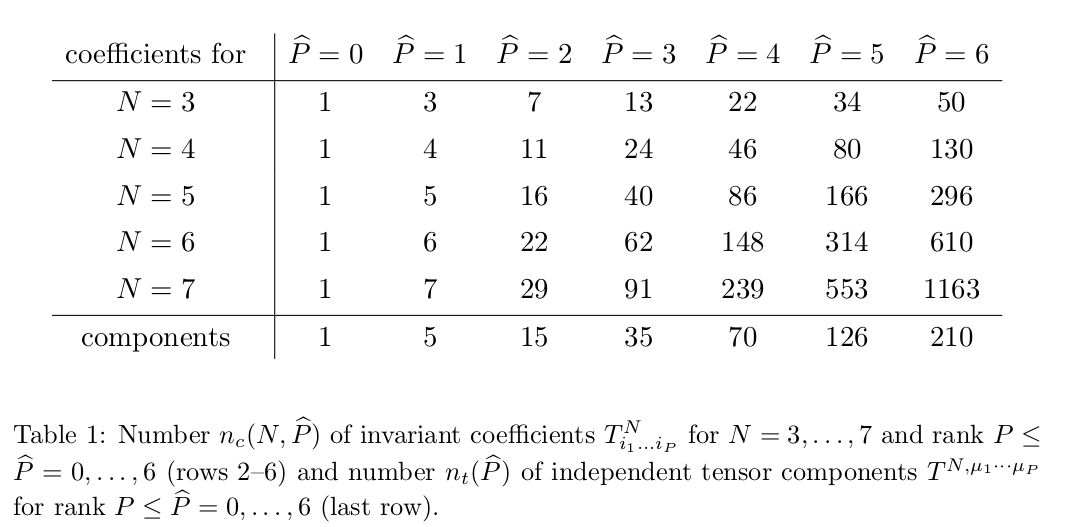
\includegraphics[scale=0.55]{pasted6}

\caption{table 1 \label{fig:table-1}}

\end{figure}

全张量积分$T^{N,\mu_{1},\cdots,\mu_{P}}$通过 type double complex 的 $4$-维数组表示,并按照以下约定

\[
\text{TNten}\left(n_{0},n_{1},n_{2},n_{3}\right)=T^{N,\overbrace{0\cdots0}^{n_{0}}\overbrace{1\cdots1}^{n_{1}}\overbrace{2\cdots2}^{n_{2}}\overbrace{3\cdots3}^{n_{3}}}
\]

按照这种方法,所有张量元$T^{N,\mu_{1},\cdots,\mu_{P}}$,其中$P=0,\ldots,\hat{P}$至一给定rank
$\hat{P}$,被存储在相同的数组中

\[
\text{double complex TNten}\left(0:\hat{P},0:\hat{P},0:\hat{P},0:\hat{P}\right)
\]

注意,全同的张量元$T^{N,\mu_{1},\cdots,\mu_{P}}$,通过一个指标的置换$\text{被\ensuremath{\left\{  \mu_{1},\ldots,\mu_{p}\right\} } }$彼此联系的,在数组
TNten 中用同一个 entry 表示。张量元$T^{N,\mu_{1},\cdots,\mu_{P}}$和数组 TNten 间的对应,在table\ref{fig:table-4}中展示,至
rank $\hat{P}=3$。

\begin{figure}
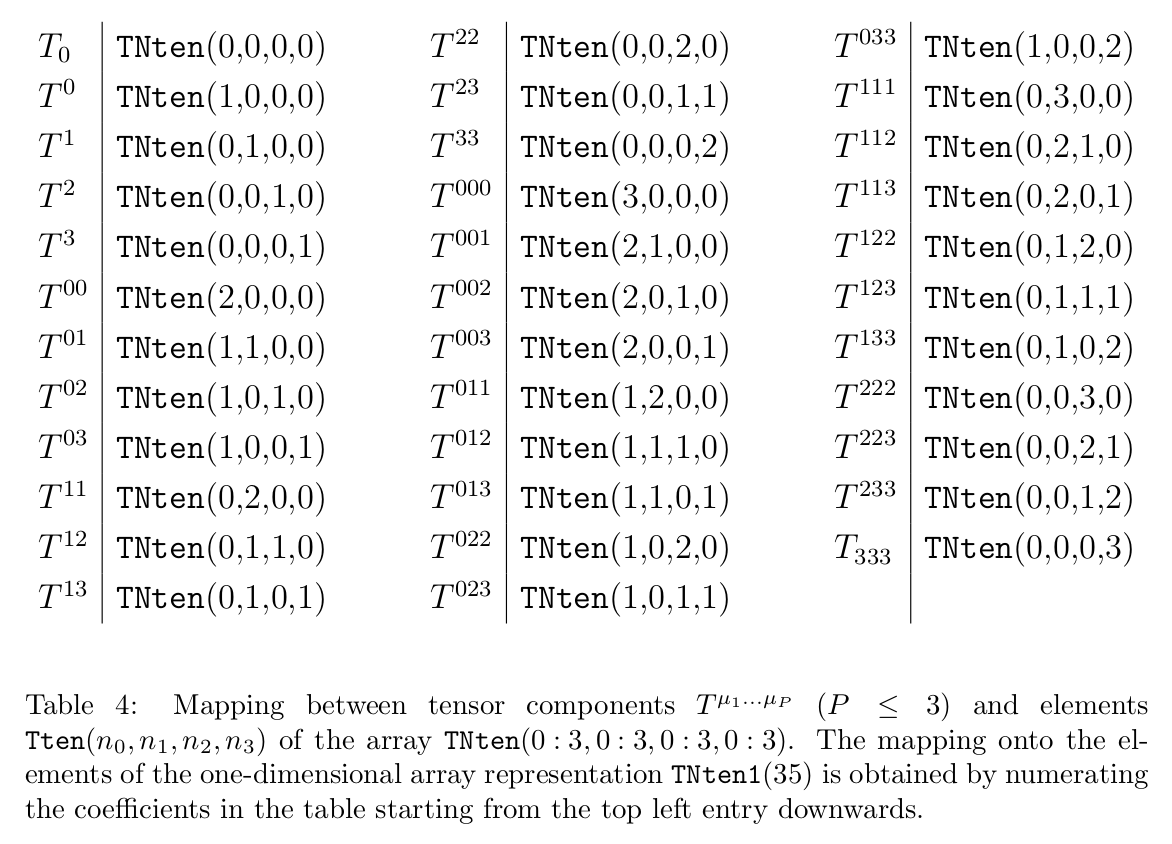
\includegraphics[scale=0.45]{pasted8}

\caption{table 4\label{fig:table-4}}

\end{figure}

洛伦兹协变分解\ref{eq:1-1}中的系数$T_{i1\cdot iP}^{N}$,来自于张量积分$T^{N,P}$,其中$N=1,\cdots,7$可以通过下列
subroutine 分别计算:A\_cll,...,G\_cll. subroutine N\_cll(N\_cll=A\_cll,...,G\_cll)
的参数结构如下给出:

subroutine N\_cll(TN,TNuv ,MomInv,mass2,R,TNerr)

double complex(0:R/2,$\underbrace{0:R,\ldots,0:R}_{N-1}$) TN : $T_{i_{1},\ldots,i_{P}}^{N,P}$with
$P\le R$

double complex(0:R/2,$\underbrace{0:R,\ldots,0:R}_{N-1}$) TNuv :
$T_{i_{1},\ldots,i_{P}}^{N,P\,\text{UV}}$with $P\le R$

double complex(1:$n_{\mathcal{P}}$) MomInv : momentum invariants

double complex(0:$N-1$) mass2 : squared masses

integer R : maximal rank

double precision(0:R) optional TNerr : error estimates

一共有$n_{\mathcal{P}}=\left(\begin{array}{c}
N\\
2
\end{array}\right)=\frac{N(N-1)}{2}=\frac{\left(N-1\right)\left(N-2\right)}{2}+\frac{2(N-1)}{2}$个动量组成的不变量$\mathcal{P}_{N}$,用符号 MomInv 表示,按照如下顺序排列:头$N$个对应$N$个 incoming
动量$k_{i}$,后面$N$个是毗连动量的和的平方$\left(k_{i}+k_{i+1}\right)^{2}$,如此等等。如果用
off-set(偏移)动量$p_{i}=k_{1}+\ldots+k_{i}$(在\ref{eq:1-1}中的传播子中出现)来写的话,将会是

\begin{align}
\mathcal{P}_{2k} & =\left(p_{1}-p_{0}\right)^{2},\left(p_{2}-p_{1}\right)^{2},\ldots,\left(p_{2k-1}-p_{2k-2}\right)^{2},\left(p_{0}-p_{2k-1}\right)^{2}\nonumber \\
 & \left(p_{2}-p_{0}\right)^{2},\left(p_{3}-p_{1}\right)^{2},\ldots,\left(p_{0}-p_{2k-2}\right)^{2},\left(p_{1}-p_{2k-1}\right)^{2},\nonumber \\
 & \ldots\nonumber \\
 & \left(p_{k-1}-p_{0}\right)^{2},\left(p_{k}-p_{1}\right)^{2},\ldots,\left(p_{k-3}-p_{2k-2}\right)^{2},\left(p_{k-2}-p_{2k-1}\right)^{2},\nonumber \\
 & \left(p_{k}-p_{0}\right)^{2},\left(p_{k+1}-p_{1}\right)^{2},\ldots,\left(p_{2k-2}-p_{k-2}\right)^{2},\left(p_{2k-1}-p_{k-1}\right)^{2},\label{eq:12}
\end{align}

\begin{align}
\mathcal{P}_{2k+1} & =\left\{ \left(p_{1}-p_{0}\right)^{2},\left(p_{2}-p_{1}\right)^{2},\ldots,\left(p_{2k}-p_{2k-1}\right)^{2},\left(p_{0}-p_{2k}\right)^{2}\right\} \nonumber \\
 & \left(p_{2}-p_{0}\right)^{2},\left(p_{3}-p_{1}\right)^{2},\ldots,\left(p_{0}-p_{2k-1}\right)^{2},\left(p_{1}-p_{2k}\right)^{2},\nonumber \\
 & \ldots\nonumber \\
 & \left(p_{k}-p_{0}\right)^{2},\left(p_{k+1}-p_{1}\right)^{2},\ldots,\left(p_{k-2}-p_{2k-1}\right)^{2},\left(p_{k-1}-p_{2k}\right)^{2},\label{eq:13}
\end{align}

注意\ref{eq:12}中的前$k-1$行每行有$N=2$个元素,第k行只有$k=N/2$个元素。而\ref{eq:13}中
k 行中每行都有$N=2k+1$个元素。

由于存在一个overall的动量守恒,$N$个incoming $ki$,但是独立的偏移量 $p_{i}$只有$N-1$个。

可以想象一个圆周,圆周上等距离的画着$N$个点,相当于两点之间连线,然后开始转动,要求两端的点不能重复。如果连线是一条直径,那么只有一半是不重复的。但是只有当圆周上的点是$2k$的时候,才可能实现这种情况。

对于$N=2,\ldots,7$,不变动量$\text{\ensuremath{\mathcal{P}}}_{N}$的集合列在
Appendix A 中。它们必须以 type double complex 提供给 subroutine N\_cll。或者是长度为
$n_{\mathcal{P}}$的数组,或者是$n_{\mathcal{P}}$个single 参数。值得注意的是,尽管变量类型是
double complex, 现版本的 COLLIER 还不支持动量不变量有虚部的情况。从长远看更重要的是,保证动量不变量的组合(对应单个外线粒子的质量平方)采用它们的精确数值,以避免任何偏差,比如对这些动量平方进行数值计算时。此外,在
IR-divergent 积分中,程序内部将会比较动量和质量参数来决定采用的解析表达式。显然,在单点积分 A\_cll中,参数 MomInv
将会省略。

squared masses 集合

\begin{equation}
\mathcal{M}_{N}=\left\{ m_{0}^{2},m_{1}^{2},\ldots,m_{N-1}^{2}\right\} \label{eq:14}
\end{equation}

进入到圈传播子中,在\ref{eq:1-1}给出,由$N$个 type double complex 的参数表示,记作 mass2。这些参数可以有不为零(负的)虚部,应当传递给
N\_ cll,格式为单个数组或者独立的参数,取决于 动量不变量 MomInv 采用的格式。

integer 参数 R 表示张量积分的最高 rank $\hat{P}$。因此它定义了输出数组 TN and TNuv 的size(type
complex)。像之前描述的,它们可以是 N-维数组,$(0:[\hat{P}/2],\left(0:P\right),\ldots\left(0:P\right)$。也可以是一维数组,长度为$n_{c}\left(N,\hat{P}\right)$。由
COLLIER 在初始化过程中表格化,可以由以下函数获取

\begin{lstlisting}
function GetNc_cll(N,R) result(nc)
integer N,R,nc:
\end{lstlisting}

integer N,R,nc:$N,\hat{P},n_{c}(N,\hat{P})$

最后,可以给出额外的输出数组TNerr ,添加$\left(0:\hat{P}\right)$个 type double precision
的 entries 到参数列表。如果存在的话,这个数组的成员传递了张量系数$T_{i1\cdot iP}^{N}$的决定误差,其中所有的$i_{k}\neq0$,对于相应的
rank $P$。误差估计 $\Delta T^{N}\left(P\right)$大概由以下方法决定:迭代计算中的误差传递,和展开式中忽略的高阶项(见
section 3.1)。返回的误差值不应该被理解为精确且可靠的,而应该被当成低层不确定性的数量级估计。

代替单独的 subroutine A\_cll,..., G\_cll, 也可以用通用 subroutine 计算任意 N的张量系数

\begin{lstlisting}
subroutine TN_cll(TN,TNuv,MomInv,mass2,Nn,R,TNerr)
\end{lstlisting}

generic TN\_cll 的参数根特定的 A\_cll,..., G\_cll 的不同仅在于 additional integer
Nn,

\begin{lstlisting}
integer Nn: # of loop propagators (=N)
\end{lstlisting}

定义了圈图中传播子的数目。在 TN\_cll 的情况下,momentum invariants \textbf{MomInv}, squared
masses \textbf{mass2},coefficients \textbf{TN}, \textbf{TNuv} 只能按照一维数组的方式处理,长度分别为$n_{\mathcal{P}},N,\text{and }n_{c}\left(N,\hat{P}\right)$。

张量元$T^{N,\mu_{1},\cdots,\mu_{P}}$with $N=1,\cdots,7$可以通过各自的 subroutine
Aten\_cll, ..., Gten\_cll 进行计算。这些 subroutine Nten\_cll 的参数结构如下

\begin{lstlisting}
subroutine
	Nten_cll(TNten, TNtenuv, MomVec, MomInv, mass2, R, Tntenerr)
\end{lstlisting}

除了 MomInv 和 mass2,跟 N\_cll 中的用法一致。这里还必须提供 $N-1$个 四矢量 $p_{i}$,就是出现在的传播子中的那些。用符号
MomVec 表示。

\begin{lstlisting}
double complex MomVec(...)
\end{lstlisting}
momentum components

可以用 $N-1$个数组表示,每个数组$\left(0:3\right)$,也可以用 单个数组,维数为$\left(0:3,N-1\right)$。注意
MomVec, MomInv, mass2 的参数形式应该一样,或者是单个数组,或者是一堆参数。和 MomInv 一样,type double
complex (尽管在现版本的COLLIER 中不支持虚部)。对于单点积分 A\_cll,MomVec参数应该省略。

整数 $R$ 代表 张量积分的最高阶 $\hat{P}$,决定了输出数组 TNten and TNtenuv 的大小(type
complex)。如同之前描述的,它们可以是$4$-维数组$\left(0:\hat{P},0:\hat{P},0:\hat{P},0:\hat{P}\right)$,或者一维数组,长度为$n_{t}\left(P\right)$。$n_{t}\left(P\right)$在
COLLIER 初始化的时候决定,可以用以下函数获得

\begin{lstlisting}
function GetNt_cll(R) result(nt)
\end{lstlisting}
 integer R,nt :$\hat{P},n_{t}(\hat{P})$

同样可以获得误差估计,通过在参数列表中提供可选的 output array TNtenerr 。它的 entries $\left(0:\hat{P}\right)$of
type precision 提供了,张量元对应 rank 绝对误差的幅值,如同在 subroutine N\_cll 中。

除了使用独立的 Aten\_cll,..., Gten\_cll ,还可以用 generic subroutine 计算张量元到任意$N$(原则上)

\begin{lstlisting}
subroutine
	TNten_cll(TNten,TNtenuv,MomVec,MomInv,mass2,Nn,R,TNtenerr).
\end{lstlisting}

TNten\_cll 跟 Aten\_cll,...,Gten\_cll 不同之处在于,多了一个 integer Nn 参数,用来指定圈图传播子的数目。

如果使用 TNten\_cll,那么 MomVec,MomInv,mass2 只能是单个数组的形式,长度为$\left(0:3,1:N-1,\right),\left(1:n_{\mathcal{P}}\right)\text{and, }\left(0:N-1\right)$,而不能是参数集合。但是输出中的Tnten
TNtenuv 用户仍然可以选择使用$\left(0:\hat{P},0:\hat{P},0:\hat{P},0:\hat{P}\right)$,或者$\left(1:n_{t}\left(P\right)\right)$的形式。

显然,不管是系数 subroutine A\_cll,..,G\_cll,TN\_cll,还是张量元subroutine Aten\_cll,...,Gten\_cll,or
TNten\_cll 的调用,都在各自的输出中,给出了相应标量积分的结果。如果用户只对标量 $1$–,...,$4$–点主积分感兴趣,可以选择限制
rank:$R=0$(i.e.$\hat{P}=0$),或者使用可选的 routines N0\_cll=A0\_cll,..,D0\_cll:

\begin{lstlisting}
subroutine N0_cll(TN0,MomInv,mass2)
\end{lstlisting}

double complex TN0: $T_{0}^{N}$.

这些 routines 提供了 标量积分的结果,输出为单个变量 TN0 of type complex,而输入 MomInv and
mass2 可以在通常的用法中作选择。注意 routines A0\_cll,...,D0\_cll 没有连接到 cache system,并且如果$3$–点函数的
Gram 行列式 和 $4$–点函数的 Cayley 行列式为零,可能会 fail。

最后, COLLIER 也提供 routines, 来计算$2$–点系数的动量导数,在对外线粒子做波函数重整化的时候会用到。需要用到的
subroutine 是 DB\_cll, 参数结构是$ $

\begin{lstlisting}
subroutine DB_cll(DB,DBuv,MomInv,mass2,R,DBerr)
double complex DB(...)
double comple DBuv(...)
double complex DBerr(...)
\end{lstlisting}

导数$B_{i_{1}\cdots i_{\hat{P}}}^{\prime}\left(p_{1}^{2}\right)\equiv\partial B_{i_{1}\cdots i_{\hat{P}}}\left(p_{1}^{2}\right)/\partial p_{1}^{2}$,的结果通过数组
DB and DBuv 返回。输入和输出参数的约定和 B\_cll 完全类似。函数 $B_{0}^{\prime},B_{1}^{\prime},B_{00}^{\prime},\text{and}B_{11}^{\prime}$可以用以下subroutines
得到,作为单个 double complex variables.

\begin{lstlisting}
subroutine DB0_cll(DB0,MomInv,mass2)
douoble complex DB0,
subroutine DB1_cll(DB0,MomInv,mass2)
douoble complex DB1,
subroutine DB00_cll(DB0,MomInv,mass2)
douoble complex DB00,
subroutine DB11_cll(DB0,MomInv,mass2)
douoble complex DB011,
\end{lstlisting}

由于导数$B_{i_{1}\cdots i_{\hat{P}}}^{\prime}\left(p_{1}^{2}\right)$没有被cached,
所以 calls of the subroutine DB\_cll, DB0\_cll, DB1\_cll, DB00\_cl,
and DB11\_cll 与 COLLIER 的缓存系统不相干。

\subsection{设置和获取参数}

张量积分的结果不仅依赖于质量和动量参数的确切值,还依赖于 regularization parameters, as well as
on technical parameters 决定约化方案的选择,和展开方法的迭代次数。最后的两组参数,对于一组确定的积分调用,通常是固定的。在
COLLIER初始化期间,它们被初始化成默认值,在\ref{fig:Table-2:-lists}中给出,并可以在稍后修改。稍后我们会给出这些参数的细节,以及使用
subroutine 改变或读取它们的值。

首先,我们注意到,COLLIER 的版本可以通过下面的 calling 获取:

\begin{lstlisting}
subroutine GetVersionNumber_cll(version)
character(len=5) version
\end{lstlisting}


\subsubsection{正规化参数}

COLLIER 使用维数正规化来处理 UV 发散。因此UV发散积分的结果依赖于\ref{eq:8}中的正规子$\Delta_{UV}$,和维数正规化能标$\mu_{UV}$,更精确地说,依赖于组合$\Delta_{UV}+\ln\left(\mu_{UV}^{2}/Q^{2}\right)$,其中
$Q^{2}$是张量积分中出现的一些能标。在微扰理论的固定阶,物理的$S$-矩阵不依赖于$\Delta_{UV}$and$\mu_{UV}$。在COLLIER中,$\Delta_{UV}$and$\mu_{UV}^{2}$被视为
type double precision 的数值参数,默认值为$\Delta_{UV}=0$and$\mu_{UV}^{2}=1$,其数值可以通过以下
subroutines 修改

\begin{lstlisting}
subroutine SetDeltaUV_cll(delta)
double precision delta,
subroutine SetMuUV2_cll(mu2)
double precision mu2
\end{lstlisting}

一方面,通过 varying 这些参数,用户数值地可以验证 $S$–矩阵元的UV有限性。另一方面,在重整化方案如 MS or $\overline{MS}$,维数重整化标度$\mu_{UV}$等同于
跑动耦合 $g\left(\mu_{ren}\right)$的重整化标度$\mu_{\text{ren}}$。在这种情况下,它具有了物理诠释,并且对
$S$–矩阵元有影响。$\Delta_{UV}$and$\mu_{UV}^{2}$值可以通过 subroutines 得到

\begin{lstlisting}
subroutine GetDeltaUV_cll(delta)
double precision delta,
subroutine GetMuUV2_cll(mu2)
double precision mu2
\end{lstlisting}

默认行为是。IR 发散也通过维数正规化。因此IR-发散的积分,其结果依赖于 $\Delta_{IR}^{\left(1\right)}$and
$\Delta_{IR}^{\left(2\right)}$defined in \ref{eq:8},and scale of
dimensional regularization, $\mu_{IR}$。在微扰理论的固定阶,IR-finite 的物理量不依赖于
$\Delta_{IR}^{\left(1\right)}$, $\Delta_{IR}^{\left(2\right)}$and
$\mu_{IR}$,一旦 virtual and real 修正被组合。在COLLIER中, $\Delta_{IR}^{\left(1\right)}$,
$\Delta_{IR}^{\left(2\right)}$and $\mu_{IR}^{2}$用 type double precision
的数值参数来表示,默认值为$\Delta_{IR}^{\left(1\right)}=\Delta_{IR}^{\left(2\right)}=0$
and $\mu_{IR}^{2}=1$,可以通过以下 subroutines 修改

\begin{lstlisting}
subroutine SetDeltaIR_cll(delta1,delta2)
double precision delta1,delta2
subroutine SetMuIR2_cll(mu2)
double precision mu2
\end{lstlisting}

注意,特别地,$\Delta_{IR}^{\left(1\right)}$and $\Delta_{IR}^{\left(2\right)}$可以被独立地改变。对$\Delta_{IR}^{\left(1\right)}$,
$\Delta_{IR}^{\left(2\right)}$and $\mu_{IR}^{2}$的variation 可以对\noun{可观测量}的IR有限性进行数值检验。现有的值可以通过以下
calling 获取

\begin{lstlisting}
subroutine GetDeltaIR_cll(delta1,delta2)
double precision delta1,delta2,
subroutine GetMuIR2_cll(mu2)
double precision mu2
\end{lstlisting}

collinear 发散也可以通过引入一列质量正规子来正规化,

\[
\mathcal{R}_{n_{reg}}=\left\{ \overline{m}_{1}^{2},\overline{m}_{2}^{2},\ldots,\overline{m}_{n_{\text{reg}}}^{2}\right\} 
\]

为了使用此功能,用户可以这样设置

\begin{lstlisting}
subroutine SetMinf2_cll(nminf,minf2)
double complex minf2(nminf)
integer nminf
\end{lstlisting}

其中 integer 变量 nminf 代表 不同正规子质量的数目 $n_{\text{reg}}$,数组 minf2 包含了 $\overline{m}_{i}^{2}$的平方值,
of type double complex。可选择地,正规子质量可以相继被添加,通过 calling the subroutine

\begin{lstlisting}
subroutine AddMinf2_cll(m2)
double complex m2
\end{lstlisting}

它让$n_{\text{reg}}$增加$1$,然后添加 double complex value m2 到列表 $\mathcal{R}_{n_{\text{reg}}}$中。当一个张量积分被调用,它的参数(质量平方和动量不变量)被数值地与$\mathcal{R}_{n_{\text{reg}}}$的元素进行比较。相同的entries
被当成无穷小 throughout the calculation,它们的数值(并不需要很小)are only kept in otherwise
singular logarithms。 在 calls of all subroutines,small masses 具有exactly
相同的值是很重要的。mass regulators 的数目 $n_{\text{reg}}$and list of squared
values can be read out with

\begin{lstlisting}
subroutine GetNminf_cll(nminf)
subroutine GetMinf2_cll(minf2)
integer nminf
\end{lstlisting}

finally, the subroutine

\begin{lstlisting}
subroutine ClearMinf2_cll
\end{lstlisting}

允许清除列表 $\mathcal{R}_{n_{\text{reg}}}$and 重置 $n_{\text{reg}}$to zero.

\subsubsection{技术参数\label{subsec:=006280=00672F=0053C2=006570}}

COLLIER 可以在三种不同模式下运行,通过

\begin{lstlisting}
subroutine SetMode_cll(mode)
integer mode
\end{lstlisting}

其中 integer argument mode=1,2,3。 For mode=1(默认值), 使用 COLI branch ,
for mode=2, the DD branch is used, for mode=3, the integrals 在两种模式下都计算。在最后一种情形下,COLLIER会返回两种结果中更好的那个。误差估计(如果在调用中指定可选参数的话)则根据两个分支的具体情况,并返回大的
那一个。COLI and DD 之间大于一定阈值的差别,将会被存储的文件 CheckOut.cll 中。mode 的值可以被获取

\begin{lstlisting}
subroutine GetMode_cll(mode)
integer mode
\end{lstlisting}

计算中设定的精度目标 $\eta_{\text{req}}$可以通过下列calling设定

\begin{lstlisting}
subroutine SetReqAcc_cll(acc)
double precision acc
\end{lstlisting}

参数 acc of type double precision。为了达到精度目标,COLLIER 会选择合适的 scheme,如果必要的话会作多种选择,展开到足够的阶。因此,$\eta_{\text{req}}$的选择决定了结果的precision和运行时间,最好权衡一下。默认值是$\eta_{\text{req}=10^{-8}}$,并且
library 对此设定进行了优化。$\eta_{\text{req}}$的当前值可以如下获得:

\begin{lstlisting}
subroutine GetReqAcc_cll(acc)
double precision acc
\end{lstlisting}

至于实际结果满足精度$\eta_{\text{req}}$的程度取决于问题的复杂度。作为第二道精度门槛,一个关键精度$\eta_{\text{crit}}$,应该比$\eta_{\text{req}}$要大,可以如下设定

\begin{lstlisting}
subroutine SetCritAcc_cll(acc)
double precision acc
\end{lstlisting}

参数 acc of type double precision。关键精度并不影响实际计算,它只是一个记账策略:如果计算的积分序列中有一个在某相空间点的不确定度达到$\eta_{\text{crit}}$,就升起一个
accuracy flag 来指示一个警告。用户可以查询这个flag,然后决定如何继续(比如放弃这个相空间点,或者改用不同的方法等等)。而且,关键的积分可以被监视。如果这个选项启用,它们的参数和结果会被自动写入到输出文件里。更多关于
accuracy flag and 监视关键积分的信息在 section 5.6 给出。关键精度被初始化为 $\eta_{\text{crit}}=10^{-1}$;它的值可以如下设定

\begin{lstlisting}
subroutine GetCritAcc_cll(acc)
double precision acc
\end{lstlisting}

最后,第三个精度参数$\eta_{\text{check}}$,应该比$\eta_{\text{req}}$大,管理COLI 和DD结果的比较。$\eta_{\text{check}}$的默认值应该是$\eta_{\text{check}}=10^{-4}$;它可以如下修改:

\begin{lstlisting}
subroutine SetCheckAcc_cll(acc)
subroutine GetCheckAcc_cll(acc)
double precision acc
\end{lstlisting}

For mode=3,如果COLI和DD的结果差距超过$\eta_{\text{check}}$,将会被记录到 file CheckOut.cll
中。mode=1 and mode=2的时候,$\eta_{\text{check}}$参数无关。

除了分别使用subroutines 设置,还可以用一个subroutine 同时设置$\eta_{\text{req}}$,$\eta_{\text{crit}}$,$\eta_{\text{check}}$,

\begin{lstlisting}
subroutine SetAccurary_cll(acc0,acc1,acc2)
double precision acc0,acc1,acc2
\end{lstlisting}

double precision arguments acc0,acc1,acc2 分别代表$\eta_{\text{req}}$,$\eta_{\text{crit}}$,$\eta_{\text{check}}$。

一个更重要的技术参数是,在迭代计算中,张量积分的最高rank $\hat{P}^{\text{max}}$,它也定义了展开方法的
cut-off order。可以如下进行设定

\begin{lstlisting}
subroutine SetRitmax_cll(ritmax)
integer ritmax
\end{lstlisting}

其中 ritmax 可以大于等于$7$。 ritmax 的值可以通过以下的方式获取

\begin{lstlisting}
subroutine GetRitmax_cll(ritmx)
\end{lstlisting}

如果对于$4$–点函数,$\hat{P}^{\text{max}}\ge7$作为最高rank,那么在内部,对于$3$–点和$2$–函数,自动设置为$\hat{P}^{\text{max}}+2$and
$\hat{P}^{\text{max}}+4$。所以如果$N\le4$,$\hat{P}^{\text{max}}$的值将会影响计算精度和时间(from
external and internal calls),library 为默认值$\hat{P}^{\text{max}}=14$特地进行了优化。注意,为了能够计算$N=N_{\text{max}}$and
$P=P_{\text{max}}$的所有张量积分$T^{N,P}$($N_{\text{max}},P_{\text{max}}$的值在初始化call
of Init\_cll 中被指定),$\hat{P}^{\text{max}}$的值不能小于$P_{\text{max}}+4-N_{\text{max}}$。

如同在 section 3 中解释的,对于$N\ge6$,约化方法既用$T_{i_{1},\ldots i_{P}}^{N}$
实现,也用$T^{N,\mu_{1}\cdots\mu_{P}}$实现了。所以当$N\ge6$时,对于一个通常的$T^{N,\mu_{1}\cdots\mu_{P}}$的计算分为3步:首先,对于$5\le\bar{N}=N_{\text{tenred}}-1\le6$,系数$T_{i_{1},\ldots i_{P_{\bar{N}}}}^{\bar{N}}$递归的从$2$–点系数开始计算。然后用$T_{i_{1},\ldots i_{P_{\bar{N}}}}^{\bar{N}}$构建$T^{\bar{N},\mu_{1}\cdots\mu_{P_{\bar{N}}}}$。最后,张量$T^{N,\mu_{1}\cdots\mu_{P}}$递归地计算自$T^{\bar{N},\mu_{1}\cdots\mu_{P_{\bar{N}}}}$,见图\ref{fig:figure1-reduction-chains}。阈值$N_{\text{tenred}}$-从何处开始张量约化,可以如下设定和获取

\begin{lstlisting}
subroutine SetTenRed_cll(Ntenred)
subroutine GetTenRed_cll(Ntenred)
integer Ntenred
\end{lstlisting}

\begin{figure}
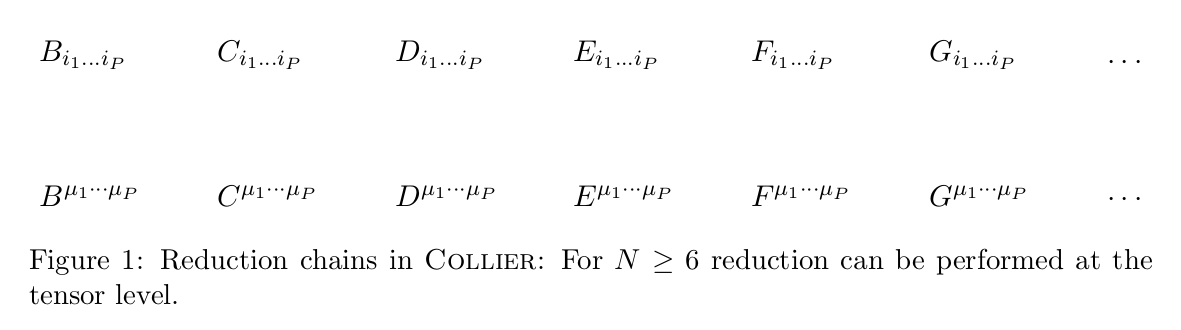
\includegraphics[scale=0.48]{pasted9}

\caption{figure1 reduction chains\label{fig:figure1-reduction-chains}}

\end{figure}

其中参数 Ntenred 代表参数$N_{\text{tenred}}$,subroutine

\begin{lstlisting}
subroutine SwitchOnTenRed_cll
\end{lstlisting}
等价于 SetTenRed\_cll(Ntenred) 并令 Ntenred=6,opts for the maximal level
of tensor reduction,而 subroutine

\begin{lstlisting}
subroutine SwitchOffTenRed_cll
\end{lstlisting}

则将它完全关闭。默认设定是maximal tensor reduction $N_{\text{tenred}}=6$,考虑到run
time 因素。

\subsection{使用缓存系统}

COLLIER 安排有 Cache 系统,避免重复计算相同的积分,以此来加快运算速度。它可以运行在 local 或者 global
mode:在local mode,仅仅在单个 subroutine call 的过程中(Section 5.3),积分被存储。cache
系统探测在约化过程中,通过不同路径到达的相同积分,然后避免它们的重复计算。在 Global 中,不同的 subroutine call
也被连接起来。local mode 总是在工作的,而 global mode 需要被显式指定。为了这个目的,也许需要创建$n_{\text{cache}}$个单独的
cache,来储存系数或者张量的结果。可以实现如下

\begin{lstlisting}
subroutine InitCacheSystem_cll(ncache,Nmax)
integer ncache, Nmax
\end{lstlisting}

其中参数 ncache and Nmax 分别代表,缓存的总数目$n_{\text{cache}}$以及计算$N$– point
积分被cached 的数目up to$N=N_{\text{cache}}^{\text{max}}$。为了启用 global mode,必须在每个计算每个相空间点之前,用
call of InitEvent(cacheNr) 把这个队列的 integral calls 分配到第 cacheNr 缓存。我们强调,对于每一个相空间点,integral
calls 必须按照相同的顺序,并且在同一个相空间点, global parameters(like $\text{\ensuremath{\mu_{\text{UV}}^{2}}}$,mode
of COLLIER 等等)不能被 reset,因为积分是依靠在用户调用序列中的次序来identified。注意对 cacheNr
的数目没有限制,需要的内存被动态分配,during the first phase-space points。取决于所解决的问题,cache
in global mode 可能会引起 hig use of memory resources。

除了在一开始固定缓存总数$n_{\text{cache}}$,还能在后续添加缓存,通过 calling of subroutine

\begin{lstlisting}
subroutine AddNewCache_cll(cache_no,Nmax)
integer cache_no,Nmax
\end{lstlisting}

新的cache,被初始化为最多储存 Nmax–点积分的结果作为输入,分配的缓存数目通过output 参数 cache\_no返回。如果之前没有初始化cache
system,call of AddNewCache\_cll 相当于 call of InitCacheSystem(ncahce=1,Nmax)。

The threshold $N_{\text{cache}}\le N_{\text{cache}}^{\text{max}}$up
to which 积分被cached,可以被单独调整,for each cache。使用如下subroutine
\begin{lstlisting}
subroutine SetCacheLevel_cll(cache_no,Nmax)
integer cache_no,Nmax
\end{lstlisting}
注意第cache\_no个缓存的level $N_{\text{cache}}^{\text{max}}$,只能在这个缓存的第一个相空间点被计算之前改变。(i.e.
在InitEvent\_cll 被首次计算之前,with the argument cache\_no)

可以使用subroutine
\begin{lstlisting}
subroutine SwitchOffCacheSystem_cll
\end{lstlisting}
暂时关闭global cache 系统。如果需要临时在integral calls序列中加入额外的call,这个选项将会很有用
\begin{lstlisting}
subroutine SwitchOnCacheSystem_cll
\end{lstlisting}
将global 缓存再次打开,将在它被中断的地方重新开始工作。

也可以之关闭一个特定的cache calling
\begin{lstlisting}
subroutine SwitchOffCache_cll(cache_no)
integer cache_no
\end{lstlisting}
在这种情况下,使用
\begin{lstlisting}
subroutine SwitchOnCache_cll(cache_no)
integer cache_no
\end{lstlisting}
再次打开。cache 在被暂停的地方重新开始,或者,如果在暂停期间 subroutine InitEvent 被调用,从缓存cache\_no积分列表中的第一个开始。

\subsection{错误处理和输出文件}

内部错误或者精度不够,在COLLIER中有两种处理方法:一方面,可以在运行过程中,设置和读取 flags for errors and
accurary;另一方面,对应的错误信息,和出错的积分calls,将会被记录在输出文件中。

error flag $\sigma_{\text{err}}$获取calling
\begin{lstlisting}
subroutine GetErrFlag_cll(errflag)
integer errflag
\end{lstlisting}

integer errflag 的值从$\sigma_{\text{err}}=0$(无错误)到$\sigma_{\text{err}}=-10$(fatal
errors)。$\sigma_{\text{err}}$保存它的值,直到被重写为更小的负数,表明遇到更加严重的错误。如此,errflag指出了它遇到的最严重的错误。当call
of InitEvent\_cll 之后,对于新相空间点的计算,它自动被重置为$\sigma_{\text{err}}=0$,也可以在任意时间重置
\begin{lstlisting}
subroutine InitErrFlag_cll
\end{lstlisting}

如果$\sigma_{\text{err}}$的值小于一个门槛$\sigma_{\text{stop}}$,程序的执行将会自动停止。默认值是$\sigma_{\text{stop}}=-8$,以使得对于相空间点的特定错误计算不会停止,而在所有相空间点出现共性错误时,停止计算。可以给$\sigma_{\text{stop}}$设置不同的值,或者获取它的值,通过给
subroutine 提供 integer argument stopflag
\begin{lstlisting}
subroutine SetErrStop_cll(stopflag),
subroutine GetErrStop_cll(stopflag)
integer stopflag
\end{lstlisting}

可以通过调用
\begin{lstlisting}
subroutine SwitchOffErrStop_cll()
\end{lstlisting}
避免程序停止。

精度flag $\sigma_{\text{acc}}$的工作方式类似。它反映了结果的精度,可以作为 integer argument
accflag 被获取
\begin{lstlisting}
subroutine GetAccFlag_cll(accflag)
integer accflag
\end{lstlisting}
初始化为$\sigma_{\text{acc}}=0$,如果没有达到$\eta_{\text{req}}$,就降为$\sigma_{\text{acc}}=-1$,如果没有达到$\eta_{\text{crit}}$,就降为$\sigma_{\text{acc}}=-2$(这些参数的细节见\ref{subsec:=006280=00672F=0053C2=006570})。想在error
flag的情形一样,$\sigma_{\text{acc}}$会被更加小的负值覆盖,来表明计算中最差的精度(从$\sigma_{\text{acc}}$被初始化之后)。call
of InitEvent\_cll for a new phase-space point 将会自动初始化$\sigma_{\text{acc}}=0$,也可以用
\begin{lstlisting}
subroutine InitAccFlag_cll
\end{lstlisting}

在初始化COLLIER的时候,用户可以选择 errors and accurary 的 messages 返回的方式。默认地,COLLIER
把它们存储在 
\begin{lstlisting}
./output_cll/
\end{lstlisting}
下的独立文件中。像在section\ref{subsec:=006982=0062EC=004F7F=007528=008BF4=00660E}中描述的,用户可以自定义输出路径,通过添加相应的字符串,作为subroutine
Init\_cll 的第二个可选参数。如果传入一个空字符串,那么相当于不创建输出文件夹。这个预定义的设置可以在随后修改,通过
\begin{lstlisting}
subroutine SwitchOffFileOutput_cll,
subroutine SwitchOnFileOutput_cll,
\end{lstlisting}
或者创建新的输出文件夹
\begin{lstlisting}
subroutine SetOutputFolder_cll(fname)
character(len=*) fname.
\end{lstlisting}
输出文件夹的名字是 fname,可以被获取
\begin{lstlisting}
subroutine GetOutputFolder_cll(fname)
character(len=*) fname
\end{lstlisting}

Error messages 被导出至 files ErrOut.coli, ErrOut.dd, and ErrOut.cll 取决于err
来自于 COLI,DD,or global接口 (or module tensors)。在初始化COLLIER的时候,这些文件被创建,一个free
output channel(number$>$100)被分配给它们。Output channel 可以被用户手动分配,通过
\begin{lstlisting}
subroutine SeterroutCOLI_cll(outchan)
subroutine SeterroutDD_cll(outchan)
subroutine Seterrout_cll(outchan)
integer outchan
\end{lstlisting}
channel number outchan 是integer 参数。尤其是,可以通过选择 outchan=6,将 error 重定向到标准channel。注意,如果文件输出被关闭,通过
subroutine SwitchOffFileOutput\_cll, standard channel 并不会被关闭,而且,重定向到标准channel(terminal或者一个专用文件)的COLLIER输出会继续传递。当前选择的输出
channel 可以如下获取
\begin{lstlisting}
subroutine GeterroutCOLL_cll(outchan)
subroutine GeterroutDD_cll(outchan)
subroutine Geterrout_cll(outchan)
integer outchan.
\end{lstlisting}
为了避免输出文件体积过大,默认的error messages 展示数目为$100$。可以通过如下更改
\begin{lstlisting}
subroutine SetMaxErrOutCOLI_cll(nout)
subroutine SetMaxErrOutDD_cll(nout)
subroutine SetMaxErrOut_cll(nout)
integer nout
\end{lstlisting}
指定对应的 integer 数目 nout 即可 。默认error 等的counters在 每次 COLLIER 重新初始化之后被重置,如果不希望重置的话,可以将
noreset=.true.传递给 Init\_cll,这些 counters 也可以手动重置
\begin{lstlisting}
subroutine InitErrCntCOLI_cll
subroutine InitErrCntDD_cll
subroutine InitErrCnt_cll
\end{lstlisting}
error 输出可以被 dis- and enabled by calling
\begin{lstlisting}
subroutine SetErrOutLev_cll(outlev)
integer outlev
\end{lstlisting}
其中 outlve=0 或者 outlev=1。如果 COLLIER 初始化的时候被传递了空数组作为输出文件夹的名字,那么 error
输出默认被关闭,其他情况都是被打开的。

额外信息和与errors无关的状态信息被记录在 log-file InfOut.cll,在初始化COLLIER时指定的目录中。同时也会有一个free
output channel(number $>100$)自动产生,并且可以被用户修改,通过传递integer outchan to
\begin{lstlisting}
subroutine Setninfout_cll(outchan)
integer outchan
\end{lstlisting}
同样允许设置为标准channel outchan=6。获得现在的channel可以用
\begin{lstlisting}
subroutine Getinfout_cll(outchan)
integer outchan
\end{lstlisting}

默认output上限是$n_{\text{inf}}^{max}=1000$,但是用户也可以修改
\begin{lstlisting}
subroutine SetMaxInfOut_cll(nout)
integer nout
\end{lstlisting}
默认情形下,$n_{\text{inf}}^{max}$以及其他的counter均会在COLLIER重新初始化期间被重置,除非设置了
noreset=.true.,作为 Init\_cll 的额外参数。informative 输出的程度可以被控制
\begin{lstlisting}
subroutine SetInfOutLev_cll(outlev)
integer outlev
\end{lstlisting}
其中的 integer argument outlev=0,1,2。用空数组作为输出文件夹时,隐含了 outlev=0(不输出),其他情况输出被设置为
outle=2(最大输出)。在后一种情况,任何内部参数的改变,都会被记录在输出文件中,可能会导致文件体积很大。比如有些参数(UV 标度
$\mu_{\text{UV}}^{2}$)被重复修改的时候(例如对于每个相空间点)。因此,也提供了折中的输出层次 outlev=1,它只追踪那些特别的活动,发生的频率较低。

当COLLIER 的模式被首次切换到 mode=3 的时候, CheckOut.cll 在通常的输出文件夹中创建。同样有相应的 channel
\begin{lstlisting}
subroutine Setncheckout_cll(outchan)
subroutine Getncheckout_cll(outchan)
integer outchan
\end{lstlisting}
在 mode=3,积分同时用library中的COLI和DD branch计算,文件 CheckOut.cll 收集这些积分的 input
and results ,如果相对偏差大于 $\eta_{\text{check}}$(见Section\ref{subsec:=006280=00672F=0053C2=006570})。$2$–点函数的导数也会被比较和保存,如果偏差大于
$\eta_{\text{check}}$。输出数目被限制到 $n_{\text{check}}^{\text{N,max}}$个问题积分和
$n_{\text{check}}^{\text{B\ensuremath{\prime},max}}$个问题导数。对于每个$N$,可以单独修改$n_{\text{check}}^{\text{N,max}}$
\begin{lstlisting}
subroutine SetMaxCheck_cll(npoints,N)
integer npoints,N
\end{lstlisting}
npoints and N代表 $n_{\text{check}}^{\text{N,max}}$和$N$。对于 $n_{\text{check}}^{\text{B\ensuremath{\prime},max}}$也是类似的
\begin{lstlisting}
subroutine SetMaxCheckDB_cll(npoints)
integer npoints
\end{lstlisting}
也可以一次性设定$n_{\text{check}}^{\text{1,max}},\cdots,n_{\text{check}}^{\text{N,max}}$,通过传递integer
array$\left\{ n_{\text{check}}^{\text{1,max}},\cdots,n_{\text{check}}^{\text{N,max}}\right\} $作为单个参数npointarray给
\begin{lstlisting}
subroutine SetMaxCheck_cll(npointarray)
integer npointarray(Nmax)
\end{lstlisting}
注意$N_{\text{max}}$的值从上次COLLIER重新初始化时,call of Init\_cll 之后就是固定的(见\ref{subsec:=006982=0062EC=004F7F=007528=008BF4=00660E})。初始值是$n_{\text{check}}^{\text{1,max}}=\cdots=n_{\text{check}}^{\text{N,max}}=n_{\text{check}}^{\text{B\ensuremath{\prime},max}}=50$。call
of Init\_cll 导致limits和counters的重新初始化,除非 noreset=.true.。更进一步的,注意 counters
for output messages in Checkout.cll 可以被手动重置为$0$,通过
\begin{lstlisting}
subroutine InitCheckCnt_cll
\end{lstlisting}
对于$N$—点积分,and
\begin{lstlisting}
subroutine InitCheckCntDB_cll
\end{lstlisting}
对于$2$–导数。

此外,用户也可以要求关于积分更详细的信息,for which 估计精度没有达到门槛$\eta_{\text{crit}}$(见\ref{subsec:=006280=00672F=0053C2=006570})这个feature必须显式开启
\begin{lstlisting}
call InitMonitoring_cll
\end{lstlisting}
激活之后,input and outputs for integrals 没有达到指定精度的,将会被记录到 CritPointsOut.cll。同样分配有
channel number
\begin{lstlisting}
subroutine Setncritpointsout_cll(outchan)
subroutine Getncritpointsout_cll(outchan)
integer outchan
\end{lstlisting}
输出被限制为头$n_{\text{crit}}^{\text{N,max}}=50$个有问题的$N$–点积分和头$n_{\text{crit}}^{\text{B\ensuremath{\prime},max}}=50$个导数.这些limits都可以更改
\begin{lstlisting}
subroutien SetMaxCritPoints_cll(npoints,N),
subroutien SetMaxCritPoints_cll(npointarray),
subroutien SetMaxCritPointsDB_cll(npoints),
integer npoints,N
integer npointarray(Nmax)
\end{lstlisting}
工作方式和 subroutine SetMaxCheck\_cll and SetMaxCheckDB\_cll 是完全相似的。初始化或者后续初始化of
COLLIER 不会改变$n_{\text{crit}}^{\text{N,max}},n_{\text{crit}}^{\text{B\ensuremath{\prime},max}}$和对应的counters。但是,call
of InitMonitoring\_cll 将重置$n_{\text{crit}}^{\text{1,max}}=\cdots=n_{\text{crit}}^{\text{N,max}}=n_{\text{crit}}^{\text{B\ensuremath{\prime},max}}=50$,相应的counters也将重置为$0$。若想只重置conunters,可以calling
\begin{lstlisting}
subroutine InitPointsCnt_cll.
\end{lstlisting}


\subsection{示例程序}

在文件夹 diretory COLLIER-$v$/build 中执行命令
\begin{lstlisting}
make demo
make democache
\end{lstlisting}
会产生两个示例程序,可以通过下面的命令执行
\begin{lstlisting}
./demo
./democache
\end{lstlisting}
in the folder COLLIER-$v$/demos

程序 demo 专门用来计算单个张量积分。在运行过程中,用户会被要求指定 mode,并在众多$N$–点积分的例子中选择一个偏爱的进行计算。计算结果写入到文件
demo\_Npoint\_exampleX.dat 中,引导用户查找到 demo.90 中各个积分的计算程序。在许多例子中,展示了同一个积分的各种调用,展示了如何与subroutine
传递参数的不同方式。例子中使用的变量定义在文件demo.f90的一开始。其中包含了很多注释,通过移除前面的感叹号,可以激活它们,以此来改变COLLIER的各种全局参数。

程序 democache 展示了缓存的使用。对1000个相空间的点集,计算了一系列共8个张量积分,并重复几次。这个玩具 Monte
Carlo 在四种配置下分别计算:使用COLI 分支,with or without cache,然后使用 DD 分支,with and
without cache。源代码放在 democache.f90 中。

\section{总结}

fortran-based library COLLIER 数值计算单圈标量或张量积分,并且对粒子的multiplicities 没有先天的限制。COLLIER的特别在于:对相空间的delicate区域,用专用技术自动优化数值稳定性,支持不稳定粒子的complex质量,对于红外发散,可以选择使用维数或质量正规化。此外,COLLIER支持检查结果的正确性和数值稳定性,由于它使用了两种独立的积分libraries,COLI
and DD。

COLLIER 可以用在传统的费曼图方法和现代的幺正性方法中。The library 已经是essential building block的代表,在自动化单圈振幅generator,如
OPENLOOPS and RECOLA,也将被更多其他生成器所使用。

\section{附录A. 动量不变量的集合,对于$N=1,...,7$}

$N$–点张量积分依赖于动量不变量$\mathcal{P}_{N}$的完整集合,$\mathcal{P}_{N}$由\ref{eq:1-1}式中传播子中的动量$p_{i}$组成。我们对集合$\mathcal{P}_{N}$中元素次序的约定在\ref{eq:12}和\ref{eq:13}中给出。为了方便,我们$N=2,\cdots,7$的$\mathcal{P}_{N}$清楚地列在这里:

\[
\mathcal{P}_{2}=\left\{ p_{1}^{2}\right\} ,
\]
\[
\mathcal{P}_{3}=\left\{ p_{1}^{2},(p_{2}-p_{1})^{2},p_{2}^{2}\right\} ,
\]
\[
\mathcal{P}_{4}=\left\{ p_{1}^{2},(p_{2}-p_{1})^{2},(p_{3}-p_{2})^{2},p_{3}^{2},p_{2}^{2},(p_{3}-p_{1})^{2}\right\} ,
\]
\begin{align*}
\mathcal{P}_{5}= & \{p_{1}^{2},(p_{2}-p_{1})^{2},(p_{3}-p_{2})^{2},(p_{4}-p_{3})^{2},p_{4}^{2},\\
 & p_{2}^{2},(p_{3}-p_{1})^{2},(p_{4}-p_{2})^{2},p_{3}^{2},(p_{1}-p_{4})^{2}\},
\end{align*}
\begin{align*}
\mathcal{P}_{6}= & \{p_{1}^{2},(p_{2}-p_{1})^{2},(p_{3}-p_{2})^{2},(p_{4}-p_{3})^{2},(p_{5}-p_{4})^{2},p_{5}^{2},\\
 & p_{2}^{2},(p_{3}-p_{1})^{2},(p_{4}-p_{2})^{2},(p_{5}-p_{3})^{2},p_{4}^{2},(p_{1}-p_{5})^{2},\\
 & p_{3}^{2},(p_{4}-p_{1})^{2},(p_{5}-p_{2})^{2}\},
\end{align*}
\begin{align*}
\mathcal{P}_{7}= & \{p_{1}^{2},(p_{2}-p_{1})^{2},(p_{3}-p_{2})^{2},(p_{4}-p_{3})^{2},(p_{5}-p_{4})^{2},(p_{6}-p_{5})^{2},p_{6}^{2},\\
 & p_{2}^{2},(p_{3}-p_{1})^{2},(p_{4}-p_{2})^{2},(p_{5}-p_{3})^{2},(p_{6}-p_{4})^{2},p_{5}^{2},(p_{1}-p_{6})^{2},\\
 & p_{3}^{2},(p_{4}-p_{1})^{2},(p_{5}-p_{2})^{2},(p_{6}-p_{3})^{2},p_{4}^{2},(p_{1}-p_{5})^{2},(p_{2}-p_{6})^{2}\}.
\end{align*}

end of file

end of file
\begin{thebibliography}{1}
\bibitem{ref61}ref61

\bibitem{ref37}ref37

\bibitem{ref50}ref50

\bibitem{ref45}ref45

\bibitem{ref52}ref52

\bibitem{ref59}ref59

\bibitem{ref43}ref43
\end{thebibliography}

\end{document}
